 \documentclass[11pt, oneside]{article} 
\usepackage{geometry}
\geometry{letterpaper} 
\usepackage{graphicx}
	
\usepackage{amssymb}
\usepackage{amsmath}
\usepackage{parskip}
\usepackage{color}
\usepackage{hyperref}

\graphicspath{{/Users/telliott_admin/Dropbox/Tex/png/}}
% \begin{center} 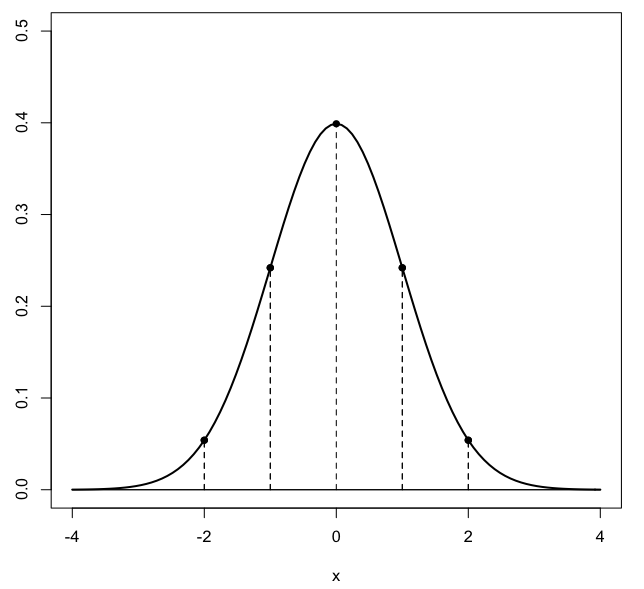
\includegraphics [scale=0.4] {gauss3.png} \end{center}

\title{Bounds and completeness}
\date{}

\begin{document}
\maketitle
\Large
An upper bound of a non-empty subset of $\mathbb{R}$ is an element $b \in \mathbb{R}$ such that $b \ge a$ for all $a \in \mathbf{A}$.

Example:  suppose $\mathbf{A}$ consists of all $x \in \mathbb{R} \ | \ x < 0$.  Then $1$ is an upper bound for $\mathbf{A}$, and so is $2$ and so is $0$.

\subsection*{completeness axiom}

If a non-empty set $\mathbf{A}$ has an upper bound, it has a least upper bound.

\subsection*{least upper bound}

An element $M \in \mathbb{R}$ is a \textbf{least upper bound} or \textbf{supremum} of $\mathbf{A}$ if 

$\circ$  $M$ is an upper bound of $\mathbf{A}$ and

$\circ$  $M \le b$ where $b$ is any other upper bound of $\mathbf{A}$.

In our example above, $0$ is the least upper bound of $\mathbf{A}$.  $0$ is the \textbf{supremum} of the set of negative real numbers.  Note that the supremum of a set is not necessarily a member of a set.

But it could be.  Suppose we replace the symbol $<$ in the definition of $\mathbf{A}$ above with $\le$.

An epsilon-delta definition says:  if $\mathbf{A}$ is bounded above with $u = sup \ \mathbf{A}$ then
\[ \forall \ \epsilon > 0 \ \exists \ x_{\epsilon} \in  \mathbf{A} \ | \  x_{\epsilon} > u - \epsilon \]

There is no "last number" before the least upper bound.  No matter how small you make $\epsilon$, one can always find $x$ whose distance from $u$ is smaller than $\epsilon$.

No matter how small is $\epsilon$ we can always find a negative number closer to zero than that.

\end{document}